\section{Statistical Methods}

We will discuss statistical methods here.  Generally, statistical methods underly questions about statistical inference which is the ability to draw conclusions from data.  There are generally three questions that we may seek to answer:
\begin{enumerate}
  \item Parameter Estimation: What is the best estimate for a parameter, $\theta$, given some data.
  \item Confidence Estimation: How confident should be be in our parameter estimation.
  \item Hypothesis testing: How consistent is a given hypothesis with the available data.
\end{enumerate}
A few of you in astronomy and physics deal with this all the time.  A few more of you deal with this as part of your job as a TA or lecturer, after all, what is a grade but a estimate of the amount of student acquired knowledge/skills. 

In this context there are two paradigms, the classical or frequentist view and the Bayesian view.  In short, the classical view is based on 
\begin{enumerate}
  \item Probabilities are related to the relative frequency of events in the world. 
  \item Parameters are fixed constants -- they don't fluctuate.
  \item All things converge in the long-run.  A 95\% confidence interval means that over the long term, the measure parameter should fall within the 95\% confidence interval, 95\% of the time.
\end{enumerate}

On the other hand, the Bayesian view is based on.
\begin{enumerate}
  \item Probability describes the degree of subjective belief -- so parameters and models can have probabilities associated with them.
  \item Inference is done by looking at the probability distribution.  Probability distributions quantify the limits of our knowledge.
\end{enumerate}

So the battle between these two paradigms can be though of as a battle between confidence and distributions.  Because distributions are functions and are more difficult to calculate, Bayesian statistics are beset by large computational requirements, something is a familiar to some of you. 

\subsection{Maximum Likelihood}

The first things we will discuss is maximum likelihood estimation.  For that we need to come up with a likelihood function:
\be
L = p(D|M(\theta))
\ee
where $L$ is the likelihood, $D$ is the data and $M(\theta)$ is a models with parameters $\theta$.  A good likelihood estimator is a Gaussian estimator:
\be
p(D|M(\theta)) = \prod_{\rm data} \frac {1}{\sqrt{\pi\sigma_i}}\exp\left(-\left(\frac{x_i - \mu_i(\theta)}{\sigma_i}\right)^2\right)
\ee
Because of the nature of exponentials, it is easier to deal with the log likelihood which is 
\be
\log(L) = -\sum_{\rm data}\left(\frac{x_i - \mu_i(\theta)}{\sigma_i}\right)^2,
\ee
where we have thrown away an additive term which is constant in $\theta$.  

The log-likelihood is the function that we have to deal with when fitting functions to data.  Here we will take two examples.  In the first case, lets assume that we have a constant error $\sigma_i=\sigma$ and lets try to fit an polynomial to it. 

Now the polynomial is already baked into numpy as it is used all the time.  However, let's do something else.  We know that the underlying function is a sine function with noise, so lets fit a sine function to it. 

In doing so we will need to compute the error.  Here the error or residuals $r_i$ are the unsquared part of the likelihood function:
\be
r_i = \frac{x_i - \mu_i(\theta)}{\sigma_i}
\ee
Note that in this case that $r_i$ can be positive and negative.  

\subsection{$\chi^2$ statistic}

Sometimes we want to see how good a model fits the data.  In this case, we can define a $\chi^2$ statistic, which is 
\be
\chi^2 = \sum_{i=1}^N\left(\frac{x_i - \mu_i(\theta)}{\sigma_i}\right)^2
\ee
where $N$ denotes the number of data points.  Now $\chi^2$ get larger and larger as the number of data points increase.  So we need to define a ``normalized'' version of $\chi^2$, which is $\chi^2{\rm dof}$ of $\chi^2$ per degree of freedom.  For a model with p parameters and N data points the number of degrees of freedom is $N-p$. So
\be
\chi_{\rm dof}^2 = \frac{1}{N-k}\sum_{i=1}^N\left(\frac{x_i - \mu_i(\theta)}{\sigma_i}\right)^2
\ee
Now if the error is distributed normally, then for a good model $\chi_{\rm dof}$ is about unity.  Much larger and this means that model likely sucks given the error.  Much smaller might indicate the we don't understand our errors or their are overestimated.  Now generally, a order unity $\chi_{\rm dof}^2$ does not mean 

Go ahead and now compute the $\chi_{\rm dof}^2$.  Is it order unity?  You should find out that it is much smaller than unity.  What does this tell you?

\subsection{Markov-Chain Monte-Carlo}

Suppose you are given some distribution of the form $P$ and you want to compute the expectation value of y.  Then the formal term is 
\be
\left<y\right> = \int y dp
\ee
Or in other words 
\be
\left<y\right> = \int y P dV,
\ee
where $V$ represents some volume in phase (state) space and $P= dp/dV$ is the probability density function.  Now lets consider the case when the state space is descrete like in quantum mechanics 
\be
\left<y\right> = \frac{\sum_i y_i P(V_i)}{\sum_i P(V_i)},
\ee
where the denominator is just ensure that the sums are properly normalized.  To make this more concrete, lets consider the case where the state space is energy $V=E$ and $P$ follows a Maxwell-Boltzman distribution.  In this case we have
\be
\left<y\right> = \frac{\sum_i y_i \exp(-E_i/k_BT)}{\sum_i \exp(-E_i/k_BT)},
\ee
where you recognized the denominator as $Z = \sum_i \exp(-E_i/k_BT)$ is the partition function from statistical mechanics.  

Suppose now we want to do this sum using monte carlo methods.  Here we cannot sum over infinite number of states but over $N$ states so we have. 
\be
\left<y\right> = \frac{\sum_{i=1}^N y_i \exp(-E_i/k_BT)}{\sum_{i=1}^N \exp(-E_i/k_BT)},
\ee
The issue is that the space of $E_i$ is huge, but for most values of $E_i$, the contribution is small e.g. $\propto \exp(-E_i/k_BT)$.  So we want to pick random values of $E_i$ following a distribution that {\it maximizes the contribution to the sum}.  To do this let consider a expectation value over a weight function $w$
\be
\left<f\right>_w = \frac{\sum_j f_j w_j}{\sum_j w_j}
\ee
Now lets define the expectation value
\be
\left<\frac{yP(E)}{w}\right>_w = \frac{\sum_j y_j P(E_j) w_j/w_j}{\sum_j w_j} = \frac{\left<y\right> Z}{\sum_j w_j}
\ee
or in other words 
\be
\left<y\right> = \left<\frac{yP(E)}{w}\right>_w Z^{-1}\sum_j w_j
\ee
Now the trick is that I will pick $w = P(E)/Z$ so that I have (when I integrate monte carlo style) 
\be
\left<y\right> = N^{-1}\sum_{i=1}^N y_i
\ee
which is simply an average over my random points, but the difficulty is that I have to pick from a distribution that follows a PDF that is defined by the weight function $w = P(E)/Z$.  I do not necessarily know how to compute the partition function as it involves as integral over all phase space.  

At the point, we will use a Markov chain, which allows us to do this integral without exact knowledge of the complete PDF.  The way is works is as follows.  
\begin{enumerate}
    \item Starting a state i, make a small change to state j.
    \item compute the transition probability $\Delta P$
    \item draw a random number $r$ in $[0,1]$ and accept the move if $r<T_{ij}$; otherwise do nothing
\end{enumerate}
In the case of the weight function that follows a Maxwell-Boltzmann distribution, the transition probability can be computed from detailed balance where 
\be
 P(E_i)R_{ij} = P(E_j)R_{ji} \rightarrow  \Delta P = \frac{R_{ij}}{R_{ji}} = \frac{P(E_j)}{P(E_i)} = \exp\left(-\frac{\Delta E_{ij}}{k_BT}\right)
\ee
where $R_{ij}$ are the rates of going from the i-th state to the j-th state

To encode all this, let us introduce the Metropolis-Hasting algorithm.  
\begin{enumerate}
    \item Starting with some state $i$
    \item Generate a set of possible moves.
    \item Pick a random move $j$ from the generate set
    \item Accept the move with probability 
    \be
    P = \min\left(1,\exp(-\frac{\Delta E_{ij}}{k_BT}\right)
    \ee
\end{enumerate}

\subsection{Bayesian Statistics}

The biggest use of MCMC is its application to model fitting especially in the context of Bayesian modeling.  Usually in this case, we are concerned about the computation of the posterior distribution function $\pi(\vec{\theta};\vec{x})$ of parameters $\vec{\theta}$ given some data $\vec{x}$ and a prior $\pi(\vec{\theta})$.  We do this via Bayes' theorem
\be
\pi(\vec{\theta};\vec{x}) = \frac{\pi(\vec{\theta})p(\vec{x};\vec{\theta})}{p(\vec{x})}
\ee
where $p(\vec{x};\vec{\theta})$ is a likelihood function and $p(\vec{x}) = \int \pi(\vec{\theta})p(\vec{x};\vec{\theta})d\vec{\theta}$ is essentially the normalization. In essence, we want to compute
\be
p(\vec{x}) = \int \pi(\vec{\theta})p(\vec{x};\vec{\theta})d\vec{\theta}
\ee
The key is that we only want to compute over the values of $\theta$ that really contribute.  So we can define a Metropolis algorithm that goes for this as
\begin{enumerate}
    \item Begin with some parameter set $\vec{\theta}_1$ 
    \item Compute the joint likelihood $L_1 = \pi(\vec{\theta}_1)p(\vec{x};\vec{\theta}_1)$
    \item Pick a random proposal $\vec{\theta}_2$ from a distribution based on the priors.
    \item Compute the likelihood $L_2 = \pi(\vec{\theta}_2)p(\vec{x};\vec{\theta}_2)$
    \item Compute the transition probability $R = L_2/L_1$
    \item Accept the proposal with probability $R$
\end{enumerate}

Lets consider the computation of the expectation values of the parameters $\vec{\theta}$ over the distribution given by the posterior distribution, $\pi(\vec{\theta};\vec{x})$ or
\be
\left<\vec{\theta}\right>_{\pi} = \int \vec{\theta}\pi(\vec{\theta};\vec{x}) d\vec{\theta} 
\ee
If I compute this value, I get the expected value of the parameters.  If I plot out $\pi(\vec{\theta})$, I get the distribution of relevant $\theta$'s 

Thus I can use MCMC for this.  A subtle, but important point is that when I take the average over the entire Markov chain, then the values of the parameters should reduce to the expected value.  However, if I take the distribution of the parameters, i.e., take a histogram of the values of the parameters in the chain, the distribution of the parameters is the posterior distribution.  This is a subtle, but important point and in case you ever wondered how these parameters distributions for various models where ever generated, now you know. 

Lets solidify our understanding with a ``simple'' example.  Let us consider our noisy sin wave as before, which we reproduce for clarity

\begin{lstlisting}[language=Python]
def generate_data() :
    A = 5
    phi = np.pi/4
    sigma = 1.0
  
    theta = np.arange(-2*np.pi, 2*np.pi, 0.025*np.pi)
    y = A*np.sin(theta + phi) + np.random.normal(0, sigma, theta.size)
  
    return theta, y, np.array([A, phi])
\end{lstlisting}  

Now we will define a log-likelihood function
\be
\log p(\vec{y}; \vec{\theta}) = -\sum_i\left(\frac{y_i - \theta_0\sin(t_i + \theta_1)}{\sigma}\right)^2,
\ee
where we set $\sigma = 1$ and $t$ is an independent variable.  We need to set some priors. Lets set $\theta_0$ to be a flat distribution between 1 and 10 and $\theta_1$ to be a flat distribution between 0 and $2\pi$.  

\begin{lstlisting}[language=Python]
def priors( x) : 
    if(x[0] < 1 or x[0] > 10) : 
      return 0
    if(x[1] < 0 or x[1] > 2*np.pi) : 
      return 0
    return 1  
\end{lstlisting}

Here is the rest of the specification.  For your HW, you will implement the heart of the algorithm, move and the loglikelihood.

\begin{lstlisting}[language=Python]
def mcmc(func, t, y, x, burn_in=1000, MAX_CHAIN=500000) :
  xchain = [] 
  i = 0

  for j in range(MAX_CHAIN) : 
    x, accepted_move = move(func, t, y, x)
    if( accepted_move) :
      i += 1 
      if( i > burn_in) : 
        xchain.append(x)
  return np.array(xchain)

def move(func, t, y, x, h = 0.1, TINY=1e-30) :
    pass

def loglikelihood( func, t, y, x, sigma=1) : 
    pass

if __name__ == "__main__" : 
    t, y, x0 = generate_data()
    guess = np.zeros(2)
    guess[0] = 2
    guess[1] = 0
    xchain = mcmc(test_function, t, y, x0)
    print( "chain length = {2} MCMC mean = {0}, actual = {1}".format(str(np.average(xchain, axis=0)), str(x0), xchain.shape[0]))
    pl.hist2d(xchain[:,0],xchain[:,1],bins=100)
    pl.show()
    pl.clf()
    pl.hist(xchain[:,0],bins=100)
    pl.savefig("mcmc_1.pdf")

\end{lstlisting}

Note that we accumulate the values of $\vec{\theta}$ as we evolve the chain and we have burn in timescale of about 1000 moves.

%\lstinputlisting[language=Python]{code/mcmc.py}

%\begin{figure}
%    \centering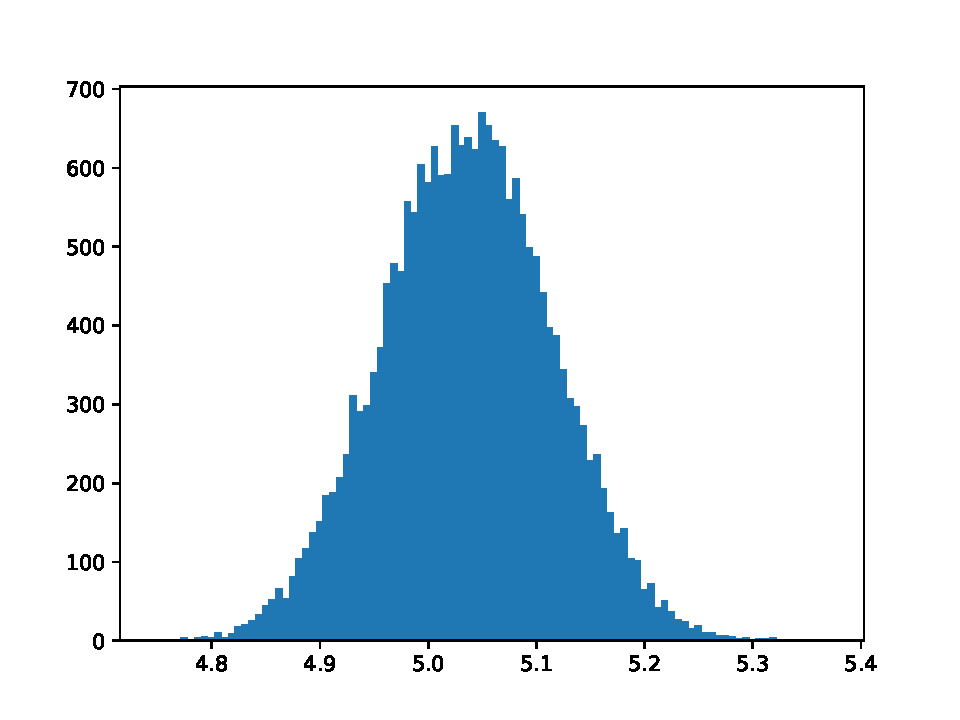
\includegraphics[width=0.75\textwidth]{code/mcmc_1.pdf}
%    \caption{\label{fig:mcmc}}
%\end{figure}

%\subsection{Simulated Annealing}



